%! Author = melek
%! Date = 9.06.2022

% Preamble
\documentclass[11pt]{article}

% Packages
\usepackage{amsmath}
\DeclareMathOperator*{\argmax}{argmax}

\usepackage{graphicx}
\usepackage{hyperref}
\graphicspath{ {../images/} }

% Document
\begin{document}

    \maketitle
    \setcounter{section}{4}


    \section{Exercises}

    \subsection{Question}
    Consider the diagrams on the right in Figure 5.1.
    Why does the estimated value function jump up for the last two rows in the rear?
    Why does it drop off for the whole last row on the left?
    Why are the frontmost values higher in the upper diagrams than in the lower?

    \subsection*{Answer}
    No answer provided.

    \subsection{Question}

    Suppose every-visit MC was used instead of first-visit MC on the blackjack task.
    Would you expect the results to be very different?
    Why or why not?

    \subsection*{Answer}

    The results would be the same because a state can be visited only once.

    \subsection{Question}

    What is the backup diagram for Monte Carlo estimation of q pi ?

    \subsection*{Answer}

    The backup diagram for MC is given at page 95.
    An empty circle and a black filled circle represent a state action pair.

    \subsection{Question}

    The pseudocode for Monte Carlo ES is inefficient because, for each state–action pair, it maintains a list of all returns and repeatedly calculates their mean.
    It would be more efficient to use techniques similar to those explained in Section 2.4 to maintain just the mean and a count (for each state–action pair) and update them incrementally.
    Describe how the pseudocode would be altered to achieve this.

    \subsection*{Answer}

    In section 2.4 average return is calculated iteratively using only current average and number of occurrences.

    Average return for each state-action pair can be calculated similarly.

    \begin{equation}
        Q(S,A) = Q(S,A) + (G - Q(S,A)) / N(S,A)
    \end{equation}

    \subsection{Question}

    Consider an MDP with a single nonterminal state and a single action that transitions back to the nonterminal state with probability p and transitions to the terminal state with probability 1-p.
    Let the reward be +1 on all transitions, and let $\gamma=1$.
    Suppose you observe one episode that lasts 10 steps, with a return of 10.
    What are the first-visit and every-visit estimators of the value of the nonterminal state?

    \subsection*{Answer}

    There is no separate behaviour policy.
    Thus importing sampling ratio is 1.

    First visit case:

    $ v(s) = 1 * 10 / 1 =  10 $

    Every visit case:

    $ v(s) = 1 * 10 + 1 * 9 + 1 * 8 + 1 * 7 + 1 * 6 + 1 * 5 + 1* 4 + 1 * 3 + 1 * 2 + 1 * 1 / 10 =  55 / 10 = 5.5 $

    Results are similar if weighted estimator is used.

    \subsection{Question}

    What is the equation analogous to (5.6) for action values Q(s, a) instead of state values V (s), again given returns generated using b?


    \subsection*{Answer}

    \begin{equation}
        Q(s,a) = \frac{\sum_{t \in \tau (s,a) } \rho_{t:(T(t)-1)} G_{t} }{ \sum_{t \in \tau (s,a) } \rho_{t:(T(t)-1)} }
    \end{equation}

    \subsection{Question}

    In learning curves such as those shown in Figure 5.3 error generally decreases with training, as indeed happened for the ordinary importance-sampling method.
    But for the weighted importance-sampling method error first increased and then decreased.
    Why do you think this happened?

    \subsection*{Answer}

    Weightet importance-sampling initially produces biased estimations.
    As the number of samples increases the bias disappears.

    \subsection{Question}

    The results with Example 5.5 and shown in Figure 5.4 used a first-visit MC method.
    Suppose that instead an every-visit MC method was used on the same problem.
    Would the variance of the estimator still be infinite? Why or why not?

    \subsection*{Answer}

    The only difference would be the added 1/k term to the sum.
    The variance would still be infinite.

    \subsection{Question}

    Modify the algorithm for first-visit MC policy evaluation (Section 5.1) to use the incremental implementation for sample averages described in Section 2.4.

    \subsection*{Answer}

    Update rule should be replaced with the following expression.

    \begin{equation}
        V(S_{t}) = V(S_{t}) + (G - V(S_{t})) / |\tau(S_{t})|
    \end{equation}

    \subsection{Question}
    \label{question:derive-update-rule-5-8}

    Derive the weighted-average update rule (5.8) from (5.7).
    Follow the pattern of the derivation of the unweighted rule (2.3).

    \subsection*{Answer}

    An important alternative is weighted importance sampling, which uses a weighted average, defined as:

    \begin{equation}
        V(s) = \frac{ \sum_{t \in \tau(s)} \rho_{t:T(t)-1} G_t }{\sum_{t \in \tau(s)} \rho_{t:T(t)-1}}
    \end{equation}

    Sequence of returns $G_1 , G_2 , \dots , G_{n-1}$ , all starting in the same state and each with a corresponding random weight $W_i$ (e.g., $ W_i = \rho_{ t_i : T (t_i)-1} $).

    \begin{equation}
        V_{n}= \frac{\sum_{k=1}^{n-1} W_{k} G_{k}}{\sum_{k=1}^{n-1} W_{k}}
    \end{equation}

    We have $C_n$ defined as :

    \begin{equation}
        C_{n}= \sum_{k=1}^{n} W_{k}
    \end{equation}

    The update rule would follow:

    \begin{equation}
        V_{n+1}=\frac{ \sum_{k=1}^{n} W_{k} G_{k}  }{ \sum_{k=1}^{n} W_{k} } = \frac{ 1 }{ \sum_{k=1}^{n} W_{k} } \sum_{k=1}^{n} W_{k} G_{k} = \frac{ 1 }{ C_{n} } ( W_{n} G_{n} +  \sum_{k=1}^{n - 1} W_{k} G_{k} )
    \end{equation}

    \begin{equation}
        V_{n+1} = \frac{ 1 }{ C_{n} } ( W_{n} G_{n} +  \frac{ \sum_{k=1}^{n-1} W_{k} }{ \sum_{k=1}^{n-1} W_{k} } \sum_{k=1}^{n - 1} W_{k} G_{k} ) = \frac{ 1 }{ C_{n} } ( W_{n} G_{n} + V_{n} \sum_{k=1}^{n-1} W_{k}  )
    \end{equation}

    \begin{equation}
        V_{n+1} = \frac{ 1 }{ C_{n} } ( W_{n} G_{n} + V_{n} (\sum_{k=1}^{n} W_{k} - W_{n}) ) = \frac{ 1 }{ C_{n} } ( W_{n} G_{n} + V_{n} (C_{n} - W_{n}) )
    \end{equation}

    \begin{equation}
        V_{n+1} = \frac{ 1 }{ C_{n} } ( W_{n} G_{n} + V_{n} C_{n} - V_{n}  W_{n} ) = \frac{ 1 }{ C_{n} } ( V_{n} C_{n} + W_{n} ( G_{n} - V_{n} ) )
    \end{equation}

    \begin{equation}
        V_{n+1} = V_{n} +  \frac{ W_{n} ( G_{n} - V_{n} ) }{ C_{n}}
    \end{equation}

    \subsection{Question}

    In the boxed algorithm for off-policy MC control, you may have been expecting the W update to have involved the importance-sampling ratio $ \frac{\pi(A_t|S_t)}{b(A_t|S_t)} $, but instead it involves $ \frac{ 1 }{b(A_t|S_t)} $ .
    Why is this nevertheless correct?

    \subsection*{Answer}

    $\pi$ is a deterministic policy ( e.g. argmax is used.).
    $ \pi $ returns 1 for the greedy action and 0 otherwise.
    The importance-sampling ratio will become 0 after policy $\pi$ and b diverges.
    As a matter of the fact, algorithm will quit the actions loop once $ A_t \neq \pi(S_t)$.

    In this setting it is OK to use 1 instead of $\pi(A_t|S_t)$ which already equals to 1.

    \subsection{Question}

    Racetrack (programming)

    Consider driving a race car around a turn like those shown in Figure 5.5. You want to go as fast as possible, but not so fast as to run off the track.

    Apply a Monte Carlo control method to this task to compute the optimal policy from each starting state.
    Exhibit several trajectories following the optimal policy (but turn the noise o↵ for these trajectories).

    \subsection*{Answer}

    \subsubsection*{Grid 1 (env2)}

    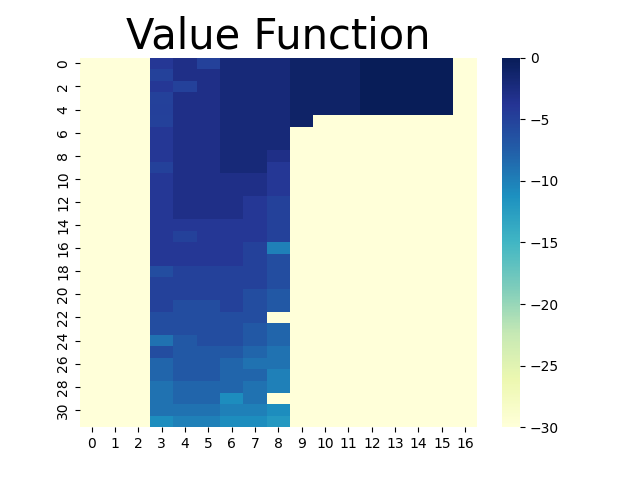
\includegraphics[scale=0.7]{env2_5_3_1_max}

    Maximum values over speeds.

    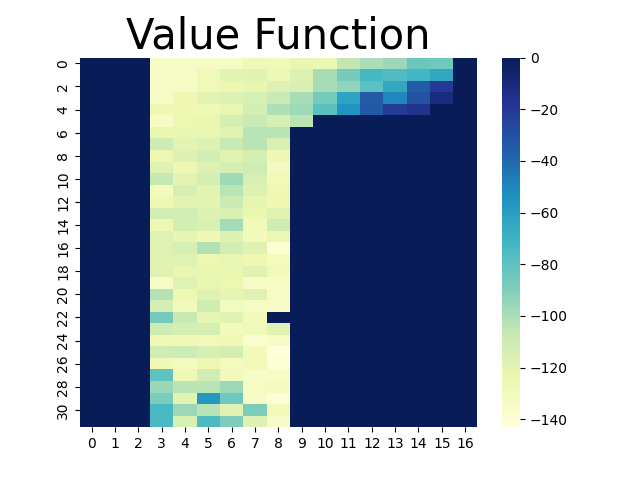
\includegraphics[scale=0.7]{env2_5_3_1_avg}

    Average values over speeds.

    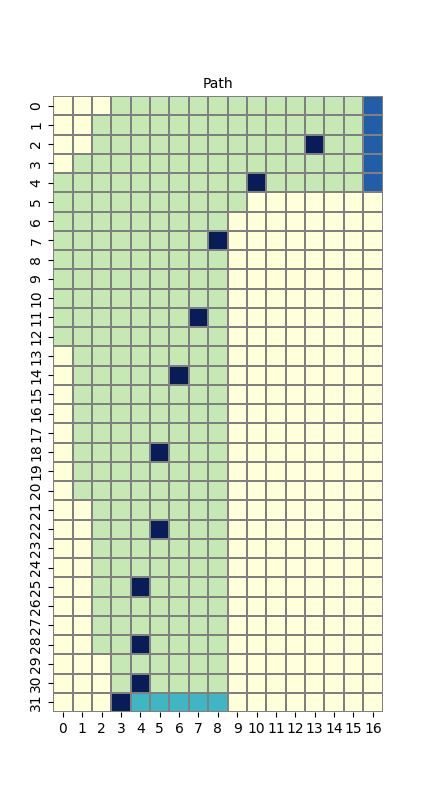
\includegraphics[scale=0.7]{env2_demo_e_5_12_3}

    Demo path.

    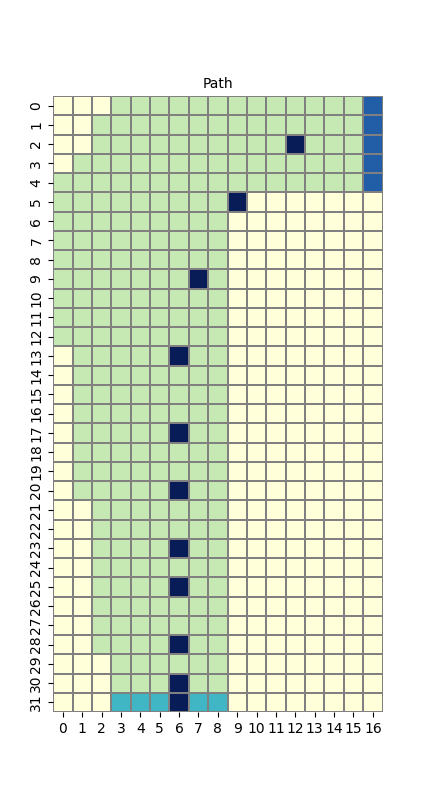
\includegraphics[scale=0.7]{env2_demo_e_5_12_6}

    Demo path.

    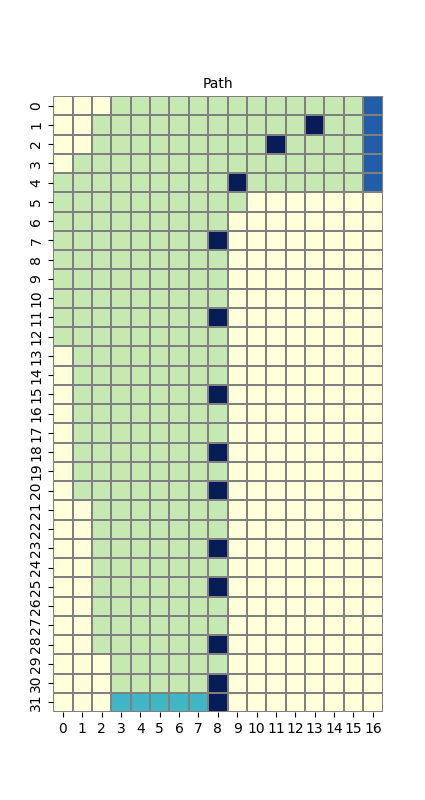
\includegraphics[scale=0.7]{env2_demo_e_5_12_8}

    Demo path.

    Average values over speeds.

    \subsubsection{Grid 2 (env3)}

    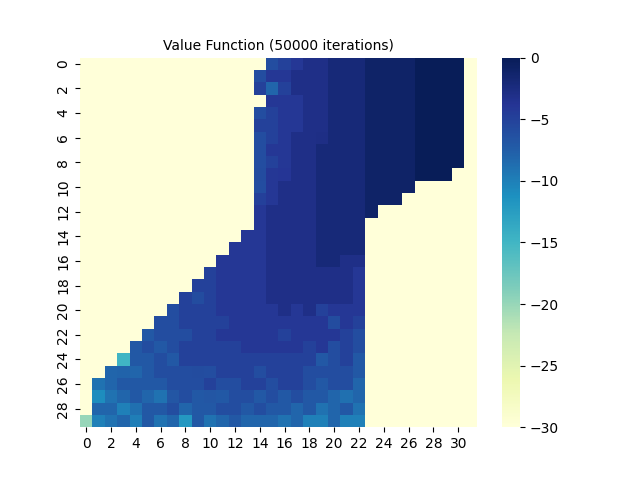
\includegraphics[scale=0.7]{env3_5_3_1_max}

    Maximum values over speeds.

    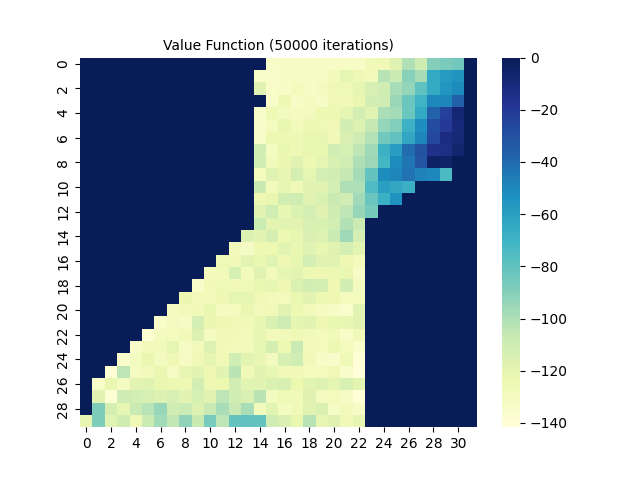
\includegraphics[scale=0.7]{env3_5_3_1_avg}

    Average values over speeds.

    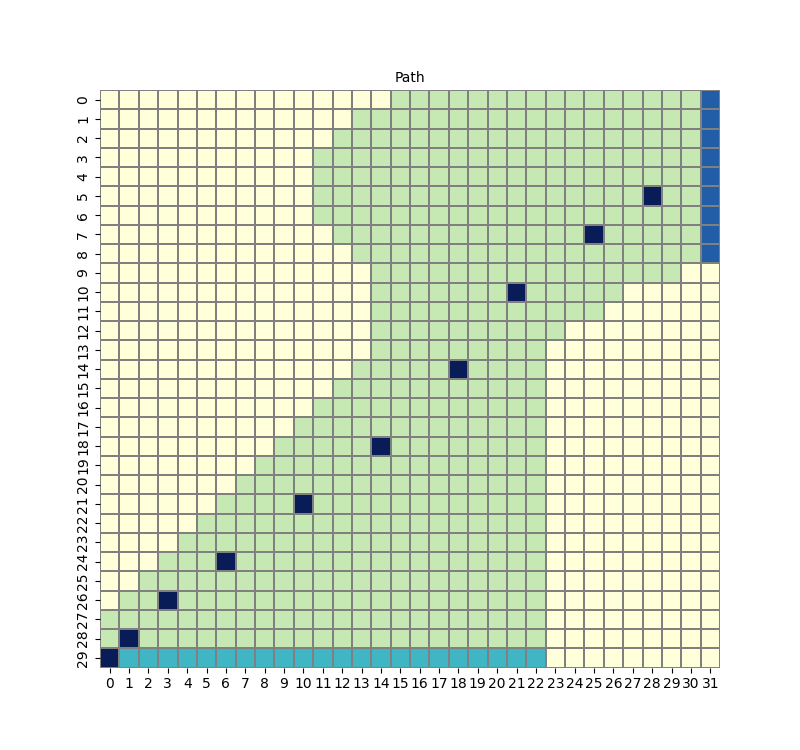
\includegraphics[scale=0.7]{env3_demo_e_5_12_0}

    Demo path.

    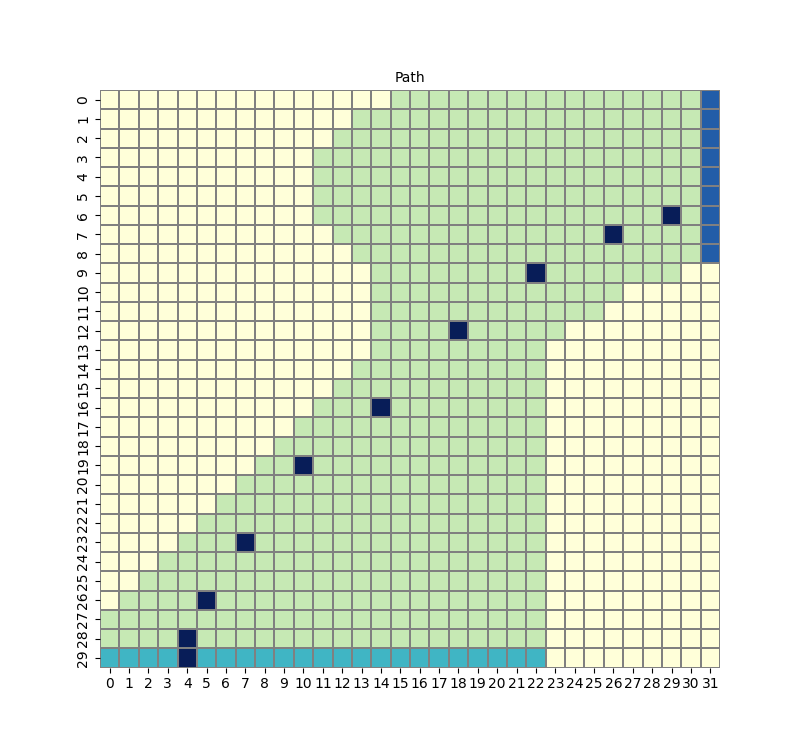
\includegraphics[scale=0.7]{env3_demo_e_5_12_4}

    Demo path.


    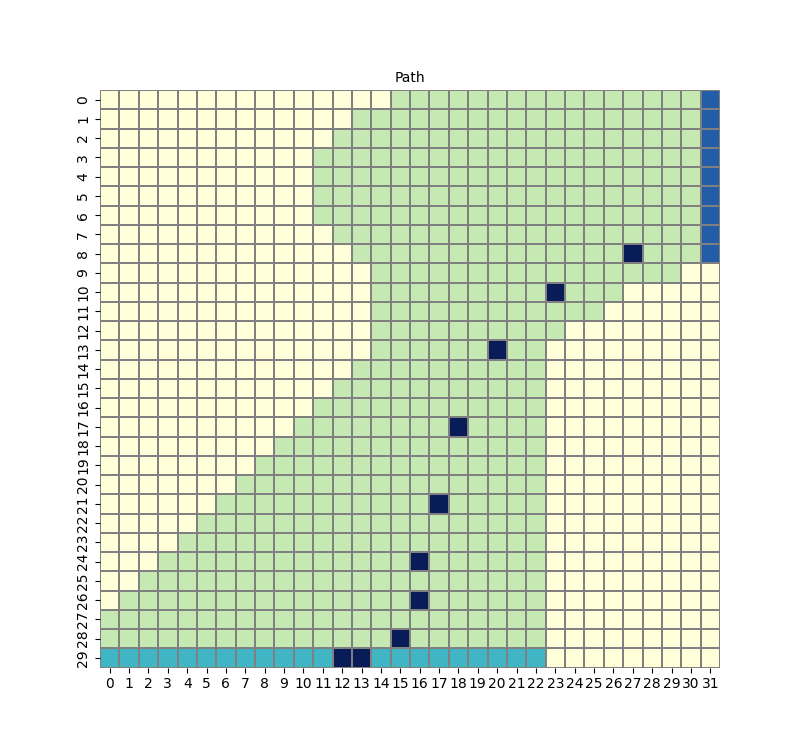
\includegraphics[scale=0.7]{env3_demo_e_5_12_12}

    Demo path.

    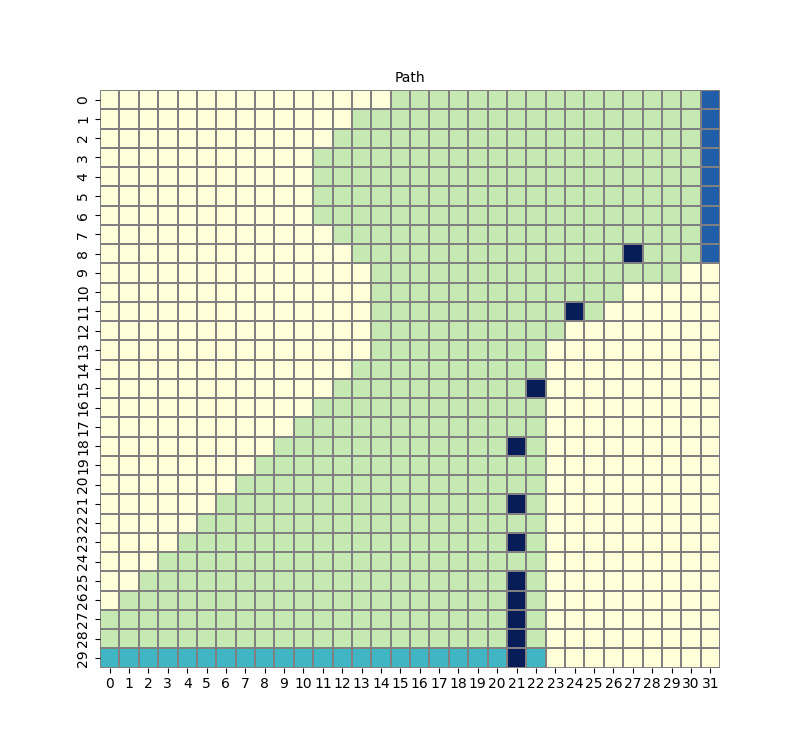
\includegraphics[scale=0.7]{env3_demo_e_5_12_21}

    Demo path.

    \subsection{Question}

    Show the steps to derive (5.14) from (5.12).

    \subsection*{Answer}

    \begin{equation}
        \rho_{t:T-1}R_{t+1} = \frac{\pi(A_t|S_t)}{b(A_t|S_t)} \frac{\pi(A_{t+1}|S_{t+1})}{b(A_{t+1}|S_{t+1})} \dots \frac{\pi(A_{T-1}|S_{T-1})}{b(A_{T-1}|S_{T-1})} R_{t+1}
    \end{equation}

    \begin{equation}
        E[\rho_{t:T-1}R_{t+1}] = E[\frac{\pi(A_t|S_t)}{b(A_t|S_t)} \frac{\pi(A_{t+1}|S_{t+1})}{b(A_{t+1}|S_{t+1})} \dots \frac{\pi(A_{T-1}|S_{T-1})}{b(A_{T-1}|S_{T-1})} R_{t+1}]
    \end{equation}

    $R_{t+1}$ depends only to time step $t$ thus we can write in $E[XY] = E[X] * E[Y]$ form.

    \begin{equation}
        E[\rho_{t:T-1}R_{t+1}] = E[\frac{\pi(A_t|S_t)}{b(A_t|S_t)} R_{t+1}] E[\frac{\pi(A_{t+1}|S_{t+1})}{b(A_{t+1}|S_{t+1})} \dots \frac{\pi(A_{T-1}|S_{T-1})}{b(A_{T-1}|S_{T-1})}]
    \end{equation}

    More over, $\pi$ or $b$ does not depend on previous timestamp.

    \begin{equation}
        E[\rho_{t:T-1}R_{t+1}] = E[\frac{\pi(A_t|S_t)}{b(A_t|S_t)} R_{t+1}] E[\frac{\pi(A_{t+1}|S_{t+1})}{b(A_{t+1}|S_{t+1})}] \dots E[\frac{\pi(A_{T-1}|S_{T-1})}{b(A_{T-1}|S_{T-1})}]
    \end{equation}

    Then we have $E[\frac{ \pi( A_{k}|S_{k} )}{ b(A_{k}|S_{k})})] = 1$


    \begin{equation}
        E[\rho_{t:T-1}R_{t+1}] = E[\frac{\pi(A_t|S_t)}{b(A_t|S_t)} R_{t+1}] * 1 \dots 1
    \end{equation}

    \begin{equation}
        E[\rho_{t:T-1}R_{t+1}] = E[\rho_{t:t}R_{t+1}]
    \end{equation}

    \subsection{Question}

    Modify the algorithm for off-policy Monte Carlo control (page 111) to use the idea of the truncated weighted-average estimator (5.10).
    Note that you will first need to convert this equation to action values.

    \subsection*{Answer}

    Weighted importance-sampling estimator:

    \begin{equation}
        V(s) =  \frac{ \sum_{t \in \tau(s) } [ (1-\gamma) \sum_{h=t+1}^{T(t)-1} \gamma^{h-t-1} \rho_{t:h-1} \bar{G}_{t:h} + \gamma^{T(t)-t-1} \rho_{t:T(t)-1} \bar{G}_{t:T(t)} ]   }{ \sum_{t \in \tau(s) } [ (1-\gamma) \sum_{h=t+1}^{T(t)-1} \gamma^{h-t-1} \rho_{t:h-1} + \gamma^{T(t)-t-1} \rho_{t:T(t)-1} ]  }
    \end{equation}

    where $\tau(s)$ is the set of all time steps in which state s is visited.
    We can turn this into action values:

    \begin{equation}
        Q(s,a) =  \frac{ \sum_{t \in \tau(s, a) } [ (1-\gamma) \sum_{h=t+1}^{T(t)-1} \gamma^{h-t-1} \rho_{t:h-1} \bar{G}_{t:h} + \gamma^{T(t)-t-1} \rho_{t:T(t)-1} \bar{G}_{t:T(t)} ]   }{ \sum_{t \in \tau(s,a) } [ (1-\gamma) \sum_{h=t+1}^{T(t)-1} \gamma^{h-t-1} \rho_{t:h-1} + \gamma^{T(t)-t-1} \rho_{t:T(t)-1} ]  }
    \end{equation}

    where $\tau(s,a)$ is the set of all time steps in which state s is visited and action a is selected.

    We can turn this expression into update rule by following steps similar to Question~\ref{question:derive-update-rule-5-8} .

    \begin{equation}
        C_{n} = \sum_{k=1}^{n} B_{k}
    \end{equation}

    \begin{equation}
        Q_{n+1} = \frac{ \sum_{k=1}^{n} A_{k}}{ \sum_{k=1}^{n} B_{k} } = \frac{ \sum_{k=1}^{n-1} A_{k} + A_{n}}{ \sum_{k=1}^{n} B_{k} } = \frac{ \frac{\sum_{k=1}^{n-1} B_{k} }{\sum_{k=1}^{n-1} B_{k} } \sum_{k=1}^{n-1} A_{k} + A_{n}}{ \sum_{k=1}^{n} B_{k} }  = \frac{ Q_{n} \sum_{k=1}^{n-1} B_{k} + A_{n}}{ \sum_{k=1}^{n} B_{k} }
    \end{equation}

    \begin{equation}
        Q_{n+1}  = \frac{1}{C_{n}} (  Q_{n} \sum_{k=1}^{n-1} B_{k} + A_{n} ) = \frac{1}{C_{n}} ( Q_{n} ( \sum_{k=1}^{n} B_{k} - B_{n} ) + A_{n} ) = \frac{1}{C_{n}} ( Q_{n} ( C_{n} - B_{n} ) + A_{n} )
    \end{equation}

    \begin{equation}
        Q_{n+1} = Q_{n} + \frac{A_{n} -  Q_{n} B_{n} }{C_{n}}
    \end{equation}

    Turn the update rule into incremental component updates.

    \subsubsection*{$C_n$ in recursive form}

    \begin{equation}
        C_{n} = C_{n+1} + B_{n+1}
    \end{equation}

    \subsubsection*{$A_n$ in recursive form}

    \begin{equation}
        A_n = \sum_{t \in \tau(s, a) } [ (1-\gamma) \sum_{h=t+1}^{T(t)-1} \gamma^{h-t-1} \rho_{t:h-1} \bar{G}_{t:h} + \gamma^{T(t)-t-1} \rho_{t:T(t)-1} \bar{G}_{t:T(t)} ]
    \end{equation}

    Where:

    \begin{equation}
        a_t = \sum_{h=t+1}^{T(t)-1} \gamma^{h-t-1} \rho_{t:h-1} \bar{G}_{t:h}
    \end{equation}

    \begin{equation}
        w_t = \rho_{t:T(t)-1}
    \end{equation}

    \begin{equation}
        \bar{G}_t = \bar{G}_{t:T(t)}
    \end{equation}

    \begin{equation}
        A_n = \sum_{t \in \tau(s, a) } [ (1-\gamma) a_t + \gamma^{T(t)-t-1} w_{t} \bar{G}_t ]
    \end{equation}

    \subsubsection*{$ B_n$ in recursive form}

    \begin{equation}
        B_n =  \sum_{t \in \tau(s,a) } [ (1-\gamma) \sum_{h=t+1}^{T(t)-1} \gamma^{h-t-1} \rho_{t:h-1} + \gamma^{T(t)-t-1} \rho_{t:T(t)-1} ]
    \end{equation}

    Where:

    \begin{equation}
        b_t = \sum_{h=t+1}^{T(t)-1} \gamma^{h-t-1} \rho_{t:h-1}
    \end{equation}

    \begin{equation}
        B_n =  \sum_{t \in \tau(s,a) } [ (1-\gamma) b_t + \gamma^{T(t)-t-1} w_{t} ]
    \end{equation}

    \subsubsection*{$b_t$ can be expanded}

    \begin{equation}
        b_t = \gamma^0 \rho_{t:t} + \gamma^1 \rho_{t:t+1} + \gamma^2 \rho_{t:t+2} + \dots + \gamma^{T-t-2} \rho_{t:T-2}
    \end{equation}

    \begin{equation}
        b_t = \gamma^0 \frac{\pi(s_{t}|a_{t})}{b(s_{t}|a_{t})} + \gamma^1 \frac{\pi(s_{t}|a_{t})}{b(s_{t}|a_{t})} \frac{\pi(s_{t+1}|a_{t+1})}{b(s_{t+1}|a_{t+1})} + \gamma^2 \frac{\pi(s_{t}|a_{t})}{b(s_{t}|a_{t})} \frac{\pi(s_{t+1}|a_{t+1})}{b(s_{t+1}|a_{t+1})} \frac{\pi(s_{t+2}|a_{t+2})}{b(s_{t+2}|a_{t+2})} + \dots
    \end{equation}

    $b_t$ can be written recursively:

    \begin{equation}
        b_t = b_{t+1} * \gamma \frac{\pi(s_{t}|a_{t})}{b(s_{t}|a_{t})} + \frac{\pi(s_{t}|a_{t})}{b(s_{t}|a_{t})} \text{ where $b_T = 0$}
    \end{equation}


    \subsubsection*{$\bar{G}_{t}$ can be written recursively}

    \begin{equation}
        \bar{G}_{t} = \bar{G}_{t:T} = R_{t+1} + \bar{G}_{t+1:T}
    \end{equation}

    \subsubsection*{$w_{t}$ can be written recursively}

    \begin{equation}
        w_{t} = \rho_{t:t} + w_{t+1}
    \end{equation}


    \subsubsection*{$a_t$ can be expanded}

    \begin{equation}
        a_t = \gamma^0 \rho_{t:t} \bar{G}_{t:t+1} + \gamma^1 \rho_{t:t+1} \bar{G}_{t:t+2} + \gamma^2 \rho_{t:t+2} \bar{G}_{t:t+3} + \dots + \gamma^{T-t-2} \rho_{t:T-2} \bar{G}_{t:T-1}
    \end{equation}

    \begin{align*}
        a_t = \gamma^0 \frac{\pi(s_{t}|a_{t})}{b(s_{t}|a_{t})} R_{t+1} + \gamma^1 \frac{\pi(s_{t}|a_{t})}{b(s_{t}|a_{t})} \frac{\pi(s_{t+1}|a_{t+1})}{b(s_{t+1}|a_{t+1})} (R_{t+1} + R_{t+2}) + \\
        \gamma^2 \frac{\pi(s_{t}|a_{t})}{b(s_{t}|a_{t})} \frac{\pi(s_{t+1}|a_{t+1})}{b(s_{t+1}|a_{t+1})} \frac{\pi(s_{t+2}|a_{t+2})}{b(s_{t+2}|a_{t+2})} (R_{t+1} + R_{t+2} + R_{t+3})+ \dots
    \end{align*}

    $a_{t}$ can be written recursively:

    \begin{equation}
        a_T = a_{T-1} = 0
    \end{equation}

    \begin{equation}
        a_{T-2} = \frac{\pi(s_{T-2}|a_{T-2})}{b(s_{T-2}|a_{T-2})} R_{T-1} = \frac{\pi(s_{T-2}|a_{T-2})}{b(s_{T-2}|a_{T-2})} ( R_{T-1} * [1] + \gamma a_{T-1} )
    \end{equation}

    \begin{equation}
        a_{T-3} = \frac{\pi(s_{T-3}|a_{T-3})}{b(s_{T-3}|a_{T-3})} ( R_{T-2} * [1 + \gamma \frac{\pi(s_{T-2}|a_{T-2})}{b(s_{T-2}|a_{T-2})}] + \gamma a_{T-2} )
    \end{equation}

    \begin{equation}
        a_{T-4} = \frac{\pi(s_{T-4}|a_{T-4})}{b(s_{T-4}|a_{T-4})} ( R_{T-3} * [1 + \gamma \frac{\pi(s_{T-3}|a_{T-3})}{b(s_{T-3}|a_{T-3})} + \gamma^2 \frac{\pi(s_{T-2}|a_{T-2})}{b(s_{T-2}|a_{T-2})} ] + \gamma a_{T-3} )
    \end{equation}

    The expression within the square brackets can be simplified to:

    \begin{equation}
        M_{t} = 1 + \sum_{k=2}^{T-t-1} \gamma^{T-t-k}  \frac{\pi(s_{T-k}|a_{T-k})}{b(s_{T-k}|a_{T-k})}
    \end{equation}

    Right side of plus one can be further simplified to:

    \begin{equation}
        m_{t} = \sum_{k=2}^{T-t-1} \gamma^{T-t-k}  \frac{\pi(s_{T-k}|a_{T-k})}{b(s_{T-k}|a_{T-k})}
    \end{equation}

    $m_{t}$ can be written recursively:

    \begin{equation}
        m_{t} = \gamma  (\frac{\pi(s_{t}|a_{t})}{b(s_{t}|a_{t})} + m_{t+1})  \text{ where $m_{T-2} = 0$}
    \end{equation}

    Final recursive expression for $a_t$ would be:

    \begin{equation}
        a_{t} = \frac{\pi(s_{t}|a_{t})}{b(s_{t}|a_{t})} ( R_{t+1} (1 + m_{t+1}) + \gamma a_{t+1})
    \end{equation}

    The final algorithm would look like:

    \subsubsection*{Initialize}

    $Q(s,a) = 0$ for all s,a. \\
    $C(s,a) = 0$ for all s,a. \\
    $ \pi(s) =a_0 $

    \subsubsection*{Loop forever}
    b=any soft policy \\
    Generate and episode using $ b: S_0 , A_0 , R_1 , \dots , S_{T-1} , A_{T-1} , R_{T} $ \\
    $ \bar{G} = R_t $ \\
    $ w = 0 $ \\
    $ a = 0 $ \\
    $ b = 0 $ \\
    $ m = 0 $

    \subsubsection*{Loop for each step $t = T-1, T-2, \dots , 0$}

    $\bar{G} = R_{t+1} + \bar{G} $ \\
    $ A =  (1-\gamma) a + \gamma^{T-t-1} w \bar{G} $ \\
    $ B =  (1-\gamma) b + \gamma^{T(t)-t-1} w  $ \\
    $ C = C + B $ \\
    $ Q = Q + \frac{A - Q B }{C} $ \\
    $ \pi(S_t) = \argmax_a Q(S_t , a) $ \\
    if $ A_t \neq \pi(S_t)$ then exit inner loop \\
    $ m = \gamma  (\frac{1}{b(s_{t}|a_{t})} + m ) $ \\
    $ a = \frac{1}{b(s_t|a_t)} ( R_{t+1} (1 + m) + \gamma a) $ \\
    $ b = b * \gamma \frac{1}{b(s_{t}|a_{t})} + \frac{1}{b(s_{t}|a_{t})} $ \\
    $ w = \frac{1}{b(s_t|a_t)} + w $
\end{document}